\documentclass[border=6pt]{standalone}
\usepackage{lmodern}
\usepackage[T1]{fontenc}
\usepackage{amsmath,amssymb}
\usepackage{bm}
\usepackage{xcolor}
\usepackage{tikz}
\usetikzlibrary{arrows.meta,positioning}
\definecolor{cgray}{HTML}{6E6C66}
\definecolor{cblue}{HTML}{2F7DC8}
\definecolor{camber}{HTML}{E0891E}
\definecolor{cgreen}{HTML}{4E8E2A}
\definecolor{cred}{HTML}{C0392B}
\definecolor{cink}{HTML}{2B2B2B}
\tikzset{>={Stealth[length=2.4mm]},
  bx/.style={rounded corners=3pt,draw=cink,line width=0.7pt,align=center,inner sep=5pt,font=\footnotesize,fill=white},
  crv/.style={line width=1.0pt,smooth,samples=120}}
\newcommand{\gau}[1]{2.0*exp(0-(#1*#1)/1.6)}
\begin{document}
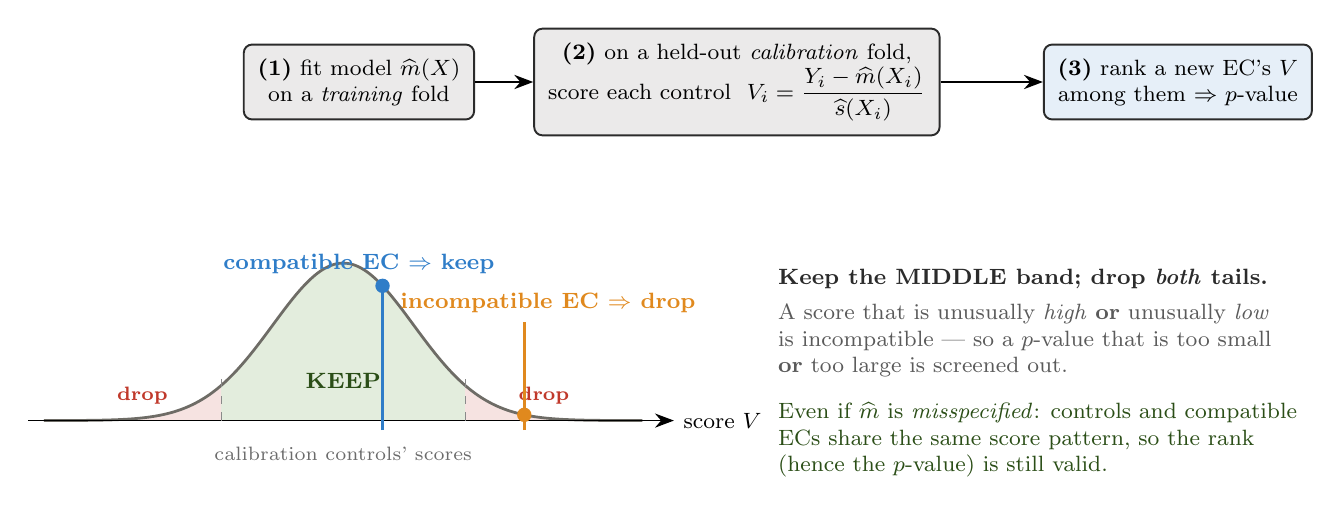
\begin{tikzpicture}[font=\small]

% ================= TOP: split-conformal flow =================
\node[bx,fill=cgray!14] (a) at (0.2,4.3) {\textbf{(1)} fit model $\widehat m(X)$\\ on a \emph{training} fold};
\node[bx,fill=cgray!14] (b) at (5.0,4.3) {\textbf{(2)} on a held-out \emph{calibration} fold,\\ score each control $\ V_i=\dfrac{Y_i-\widehat m(X_i)}{\widehat s(X_i)}$};
\node[bx,fill=cblue!12] (c) at (10.6,4.3) {\textbf{(3)} rank a new EC's $V$\\ among them $\Rightarrow$ $p$-value};
\draw[->,line width=0.9pt] (a) -- (b);
\draw[->,line width=0.9pt] (b) -- (c);

% ================= BOTTOM: the calibration-score distribution =================
\def\q{1.55}
\fill[cgreen!16] (-\q,0) -- plot[domain=-\q:\q,samples=60] (\x,{\gau{\x}}) -- (\q,0) -- cycle;
\fill[cred!14] (\q,0) -- plot[domain=\q:3.7,samples=40] (\x,{\gau{\x}}) -- (3.7,0) -- cycle;
\fill[cred!14] (-3.7,0) -- plot[domain=-3.7:-\q,samples=40] (\x,{\gau{\x}}) -- (-\q,0) -- cycle;
\draw[crv,cgray] plot[domain=-3.8:3.8] (\x,{\gau{\x}});
\draw[->] (-4.0,0) -- (4.2,0) node[right,font=\footnotesize]{score $V$};
\draw[cink!55,dashed] (\q,0) -- (\q,{\gau{\q}+0.15}); \draw[cink!55,dashed] (-\q,0) -- (-\q,{\gau{-\q}+0.15});
\node[cgreen!55!black,font=\footnotesize\bfseries] at (0,0.5) {KEEP};
\node[cred,font=\scriptsize\bfseries] at (2.55,0.32) {drop}; \node[cred,font=\scriptsize\bfseries] at (-2.55,0.32) {drop};
\node[font=\scriptsize,cink!70] at (0,-0.42) {calibration controls' scores};
% example ECs
\draw[cblue,line width=1.2pt] (0.5,-0.12) -- (0.5,{\gau{0.5}}); \fill[cblue] (0.5,{\gau{0.5}}) circle (2.6pt);
\node[cblue,font=\footnotesize\bfseries,anchor=south] at (0.2,{\gau{0.5}+0.03}) {compatible EC $\Rightarrow$ keep};
\draw[camber,line width=1.2pt] (2.3,-0.12) -- (2.3,1.25); \fill[camber] (2.3,{\gau{2.3}}) circle (2.6pt);
\node[camber,font=\footnotesize\bfseries,anchor=south] at (2.6,1.25) {incompatible EC $\Rightarrow$ drop};

% ================= right message =================
\node[cink,font=\footnotesize\bfseries,anchor=north west] at (5.4,2.05) {Keep the MIDDLE band; drop \emph{both} tails.};
\node[cink!78,font=\footnotesize,anchor=north west,align=left] at (5.4,1.6)
   {A score that is unusually \emph{high} \textbf{or} unusually \emph{low}\\ is incompatible --- so a $p$-value that is too small\\ \textbf{or} too large is screened out.};
\node[cgreen!55!black,font=\footnotesize,anchor=north west,align=left] at (5.4,0.35)
   {Even if $\widehat m$ is \emph{misspecified}: controls and compatible\\ ECs share the same score pattern, so the rank\\ (hence the $p$-value) is still valid.};

\end{tikzpicture}
\end{document}
